\appendix
\renewcommand{\thesection}{\Alph{section}}

\section{Eliminating dimensions} \label{appendix:elim_dim}

As described in \secref{sec:choice_of_systems}, we will prefer to deal with energy units of either $\hbar \omega$ or $\hbar$ and lenght units of $a_{ho} = \sqrt{\hbar/m\omega}$. We now show how this allows us to write the simplified Hamiltonian expressions. Starting from the noninteractive part of the Hamiltonian,
\begin{equation*}
    \hat{H}_0=\sum_i^N \left(\frac{-\hbar^2}{2m}{\nabla }_{i}^2 +\frac{1}{2}m\omega^2r_i^2\right), 
\end{equation*}
we make a change of coordinates $r\to r/a_{ho}$ so that the Cartesian coordinates become $\hat{x}_i = x_i/a_{ho}$ and the components of the gradient vector undergo the change of coordinates
 \begin{equation*}
     \frac{\partial }{\partial \hat{x}_i} =\frac{\partial }{\partial \hat{x}_i}\frac{\partial \hat{x}_i}{\partial x_i} = \frac{1}{a_{ho}}\frac{\partial }{\partial \hat{x}_i},
\end{equation*}
which naturally propagate to the Laplacian as
 \begin{equation*}
     {\hat{\nabla} }_{i}^2 = \frac{1}{a_{ho}^2}{\nabla }_{i}^2.
\end{equation*}

Now, in the new coordinate system, but going back to the original notation not to pollute the demonstration, the Hamiltonian turns into 
 \begin{equation*}
     \hat{H}_0 = \sum_i^N -\frac{\hbar}{2m}\frac{1}{a_{ho}^2}{\nabla }_{i}^2 + \frac{m}{2}\left(\omega r_i/a_{ho} \right)^2.
\end{equation*}

Using the definition of $a_{ho}$, some terms simplify giving 
 \begin{equation*}
     \hat{H}_0 = \sum_i^N -\frac{\hbar\omega}{2}{\nabla }_{i}^2 + \frac{\hbar\omega}{2}r_i^2.
\end{equation*}

Finally, by using energy units of $\hbar \omega$,
 \begin{equation*}
     \frac{\hat{H}_0}{\hbar \omega} = \sum_i^N -\frac{1}{2}{\nabla }_{i}^2 + \frac{1}{2}r_i^2.
\end{equation*}

Now for the interactive part of the Hamiltonian, we have two scenarios. For the Coulomb interaction, can use an arbitrary unit of charge such that 
 \begin{equation*}
    \sum_{i< j} V_{int}(\mathbf{r}_i, \mathbf{r}_j)= \frac{1}{4\pi \epsilon_0}\sum_{i < j} \frac{q_iq_j}{r_{ij}} \to \sum_{i < j} \frac{1}{r_{ij}},
\end{equation*}
where $\epsilon_0$ is the permittivity of free space, and $q_i$ the charge of particle $i$.

For the finite range interaction, we redefine the interaction range $\sigma_0 = \sigma/a_{ho}$ and the interaction strength $V_o = V/(a_{ho}\hbar\omega)$
\begin{align*}
    \sum_{i< j} V_{int}(\mathbf{r}_i, \mathbf{r}_j)= \frac{V}{\sigma \sqrt{2\pi}}\sum_{i< j} \exp\left[-\frac{r_{ij}^2}{2 \sigma^2}\right] \to \frac{V_0 (a_{ho}\hbar\omega)}{\sigma_0 a_{ho} \sqrt{2\pi}}\sum_{i< j} \exp\left[-\frac{a_{ho}^2 r_{ij}^2}{2 a_{ho}^2\sigma_0^2}\right],
\end{align*}
Which finally, in energy units of $\hbar \omega$ becomes
\begin{align*}
    \sum_{i< j} V_{int}(\mathbf{r}_i, \mathbf{r}_j)= \frac{V_0 }{\sigma_0 \sqrt{2\pi}}\sum_{i< j} \exp\left[-\frac{ r_{ij}^2}{2 \sigma_0^2}\right].
\end{align*}


\section{VMC derivations}\label{appendix:vmc}

Let $f(\mvec{r})=\ln{\Psi}(\mvec{r})$ and $E_L = K_L + V_L$. Note then that  

\begin{align}
    \nabla f(\mvec{r}) &= \frac{\nabla \Psi(\mvec{r})}{\Psi(\mvec{r})} \\
    \nabla^2 f(\mvec{r}) &=  \frac{\nabla^2 \Psi(\mvec{r})}{\Psi(\mvec{r})} - \left(  \frac{\nabla \Psi(\mvec{r})}{\Psi(\mvec{r})}\right)^2,
\end{align}
which leads to 
\begin{align}
    K_L(\mvec{r}) &= -\frac{1}{2}\frac{ \nabla^2 \Psi(\mvec{r})}{\Psi(\mvec{r})} \\
    & = -\frac{1}{2} \left(\nabla^2 f(\mvec{r}) +  \left( \nabla f(\mvec{r})\right)^2 \right).
\end{align}



\section{Steepest descent derivations}\label{appendix:steepest}

We posed the steepest descent problem as the constrained optimisation of minimising
\begin{align*}
\quad \mathcal{L}(\mvec{\theta}_{t}) + (\mvec{\theta} - \mvec{\theta}_t)^\top \nabla \mathcal{L}(\mvec{\theta}_{t}) + \frac{1}{2} \| \mvec{\theta} - \mvec{\theta}_t \|_2^2,
\end{align*}
subject to $\| \mvec{\theta} - \mvec{\theta}_t \|_2 = \epsilon$.

For that we introduce a Lagrange multiplier $\lambda$ to incorporate the constraint into the objective function, leading to the Lagrangian:
\begin{align*}
\mathcal{G}(\mvec{\theta}, \lambda) = \mathcal{L}(\mvec{\theta}_{t}) + (\mvec{\theta} - \mvec{\theta}_t)^\top \nabla \mathcal{L}(\mvec{\theta}_{t}) + \frac{1}{2} \| \mvec{\theta} - \mvec{\theta}_t \|_2^2 + \lambda \left( \| \mvec{\theta} - \mvec{\theta}_t \|_2 - \epsilon \right).
\end{align*}

Taking derivatives with respect to \( \mvec{\theta} \) and \( \lambda \), and seting them to zero, we have
\begin{align*}
\nabla_{\mvec{\theta}} \mathcal{G}(\mvec{\theta}, \lambda) &= \nabla \mathcal{L}(\mvec{\theta}_{t}) + (\mvec{\theta} - \mvec{\theta}_t) + \lambda \frac{\mvec{\theta} - \mvec{\theta}_t}{\| \mvec{\theta} - \mvec{\theta}_t \|} = 0,    \\
\frac{\partial \mathcal{G}}{\partial \lambda} &= \| \mvec{\theta} - \mvec{\theta}_t \| - \epsilon = 0.
\end{align*}

The gradient with respect to $\lambda$ simply enforces the constrain, $\| \mvec{\theta} - \mvec{\theta}_t \| = \epsilon$, but from the gradient with respect to $ \mvec{\theta} $ we find
\begin{align*}
(\mvec{\theta} - \mvec{\theta}_t)(1 +  \frac{\lambda}{\| \mvec{\theta} - \mvec{\theta}_t \|}) = - \nabla \mathcal{L}.
\end{align*}

Here we could further investigate the $\lambda$ factor, but the important thing is that this yields
\begin{align*}
\mvec{\theta}_{t+1} = \mvec{\theta}_t - \alpha \nabla \mathcal{L}(\mvec{\theta}_{t}), 
\end{align*}
for some $\alpha$ that depends on the constraint $\epsilon$.

\section{Gaussian-binary RBM expressions}\label{appendix:rbm}

The marginal probability distribution for the Gaussian-binary RBM's visible nodes is given by
\begin{align*}
p(\vec{R}) = \exp\left\{-\sum_i^{n_r} \frac{(r_i - a_i)^2}{2\sigma^2}\right\}\sum_{\{\mvec{h}\}} \exp\left\{\sum_j^{n_h} b_j h_j +\sum_{i,j}^{n_r,{n_h}} \frac{r_i w_{ij} h_j}{\sigma^2} \right\},
\end{align*}
where we can rewrite the summation over all possible vectors $\mvec{h}$ as
\begin{align*}
\sum_{\{h\}} \exp \left( \sum_{j} \left( b_j + \sum_{i} \frac{r_i w_{ij}}{\sigma^2} \right) h_j \right).
\end{align*}
Now, if we denote for simplicity:
\begin{align*}
\theta_j = b_j + \sum_{i} \frac{r_i w_{ij}}{\sigma^2},
\end{align*}
the expression becomes
\begin{align*}
\sum_{\{h\}} \exp \left( \sum_{j} \theta_j h_j \right)&= \prod_{j} \left( \sum_{h_j=0}^{1} \exp (\theta_j h_j) \right) \\
&=\prod_{j} \left( 1 + \exp (\theta_j) \right).
\end{align*}
Substituting back $\theta_j$ gives us
\begin{align*}
p(\vec{R}) = \exp\left\{-\sum_i^{n_r} \frac{(r_i - a_i)^2}{2\sigma^2}\right\}\prod_{j} \left[ 1 + \exp \left\{ b_j + \sum_{i} \frac{r_i w_{ij}}{\sigma^2} \right\} \right].
\end{align*}

\section{Minimal Running NQS Script}\label{sec:minimal_nqs}

We here provide a minimal example for a simulation script for running an NQS simulation. The configurations, of course, have to be set up correctly in a yaml file which has to be passed as argument.

\begin{lstlisting}[caption={Simplified example of execution code for a NQS experiment}, label={lst:nqs_code}]
import argparse, os, jax, yaml
import numpy as np
from nqs.state import nqs

def initialize_system(config):
    system = nqs.NQS(
        backend=config["backend"],
        logger_level="INFO",
        seed=config["seed"],
    )

    common_kwargs = {
        "correlation": config["correlation"],
        "particle": config["particle"],
        "nhidden": config.get("nhidden"),
        "sigma2": 1.0 / np.sqrt(config["omega"]) if config["nqs_type"] != "dsffn" else None
    }
    config["common_kwargs"] = common_kwargs
    system.set_wf(config["nqs_type"], config["nparticles"], config["dim"], **common_kwargs)
    return system

def run_experiment(config):
    system = initialize_system(config)
    system.set_sampler(
        mcmc_alg=config["mcmc_alg"],
        scale=1 / np.sqrt(config["nparticles"] * config["dim"]),
    )
    system.set_hamiltonian(
        type_="ho",
        int_type=config["interaction_type"],
        omega=config["omega"],
        r0_reg=10,
        training_cycles=config["training_cycles"],
    )
    system.set_optimizer(
        optimizer=config["optimizer"],
        eta=config["eta"] / np.sqrt(config["nparticles"] * config["dim"]),
    )

    if config["nqs_type"] == "dsffn":
        system.pretrain(
            model="Gaussian",
            max_iter=1000,
            batch_size=2000,
            logger_level="INFO",
            args=config["common_kwargs"],
        )

    history = system.train(
        max_iter=config["training_cycles"],
        batch_size=config["batch_size"],
        early_stop=False,
        history=True,
        tune=False,
        grad_clip=0,
        seed=config["seed"],
    )

    df_samples = system.sample(
        config["nsamples"],
        config["nchains"],
        config["seed"],
        save_positions=config["save_positions"],
    )

def load_config(config_path):
    with open(config_path, "r") as file:
        return yaml.safe_load(file)

if __name__ == "__main__":
    parser = argparse.ArgumentParser(description="Run NQS Experiment")
    parser.add_argument("--config", type=str, required=True, help="Path to the configuration file")
    args = parser.parse_args()

    config_path = os.path.join(os.path.dirname(__file__), args.config)
    run_experiment(load_config(config_path))
\end{lstlisting}

\section{Additional Results 1D Case}\label{apendix:more_results_1d}

\begin{figure}[H]
    \centering
    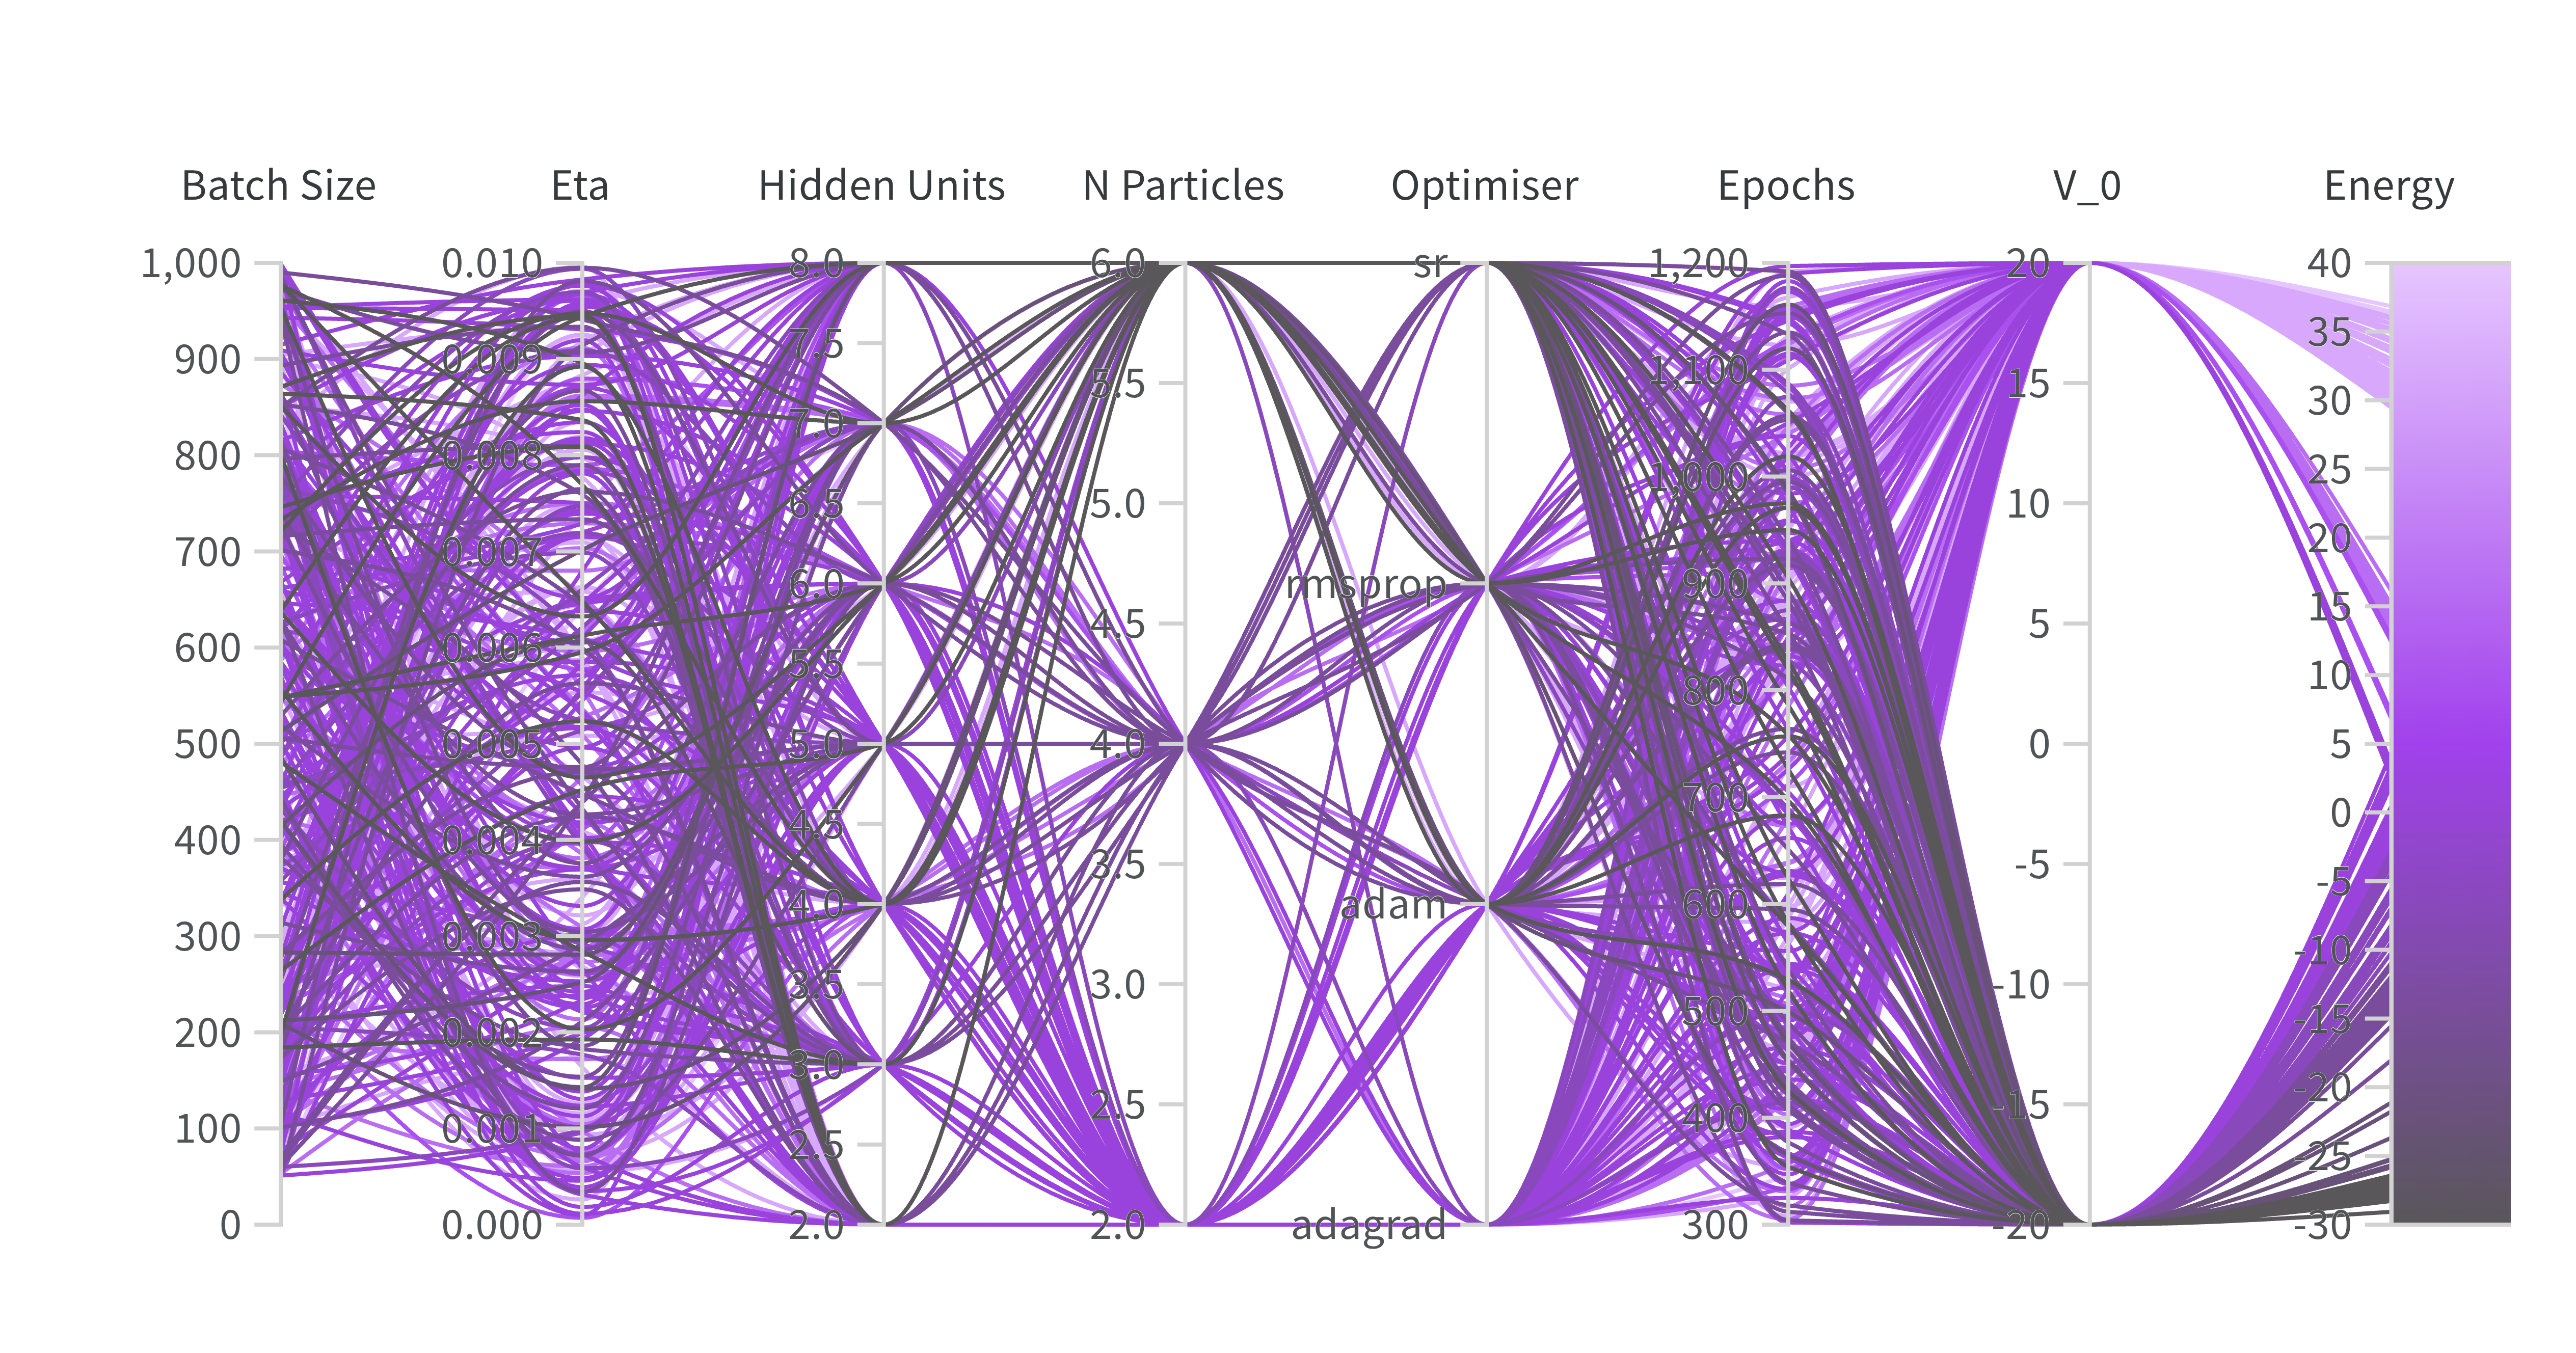
\includegraphics[width=0.8\linewidth]{Chapters/Results/N2/rbm_sweep.png}
    \caption{Sweep over 324 hyperparameters for the standard RBM ansatz, from which the results shall be aggregated for the one-dimensional system.}
    \label{fig:vmc_complete_sweep}
\end{figure}
\begin{figure}[H]
    \centering
    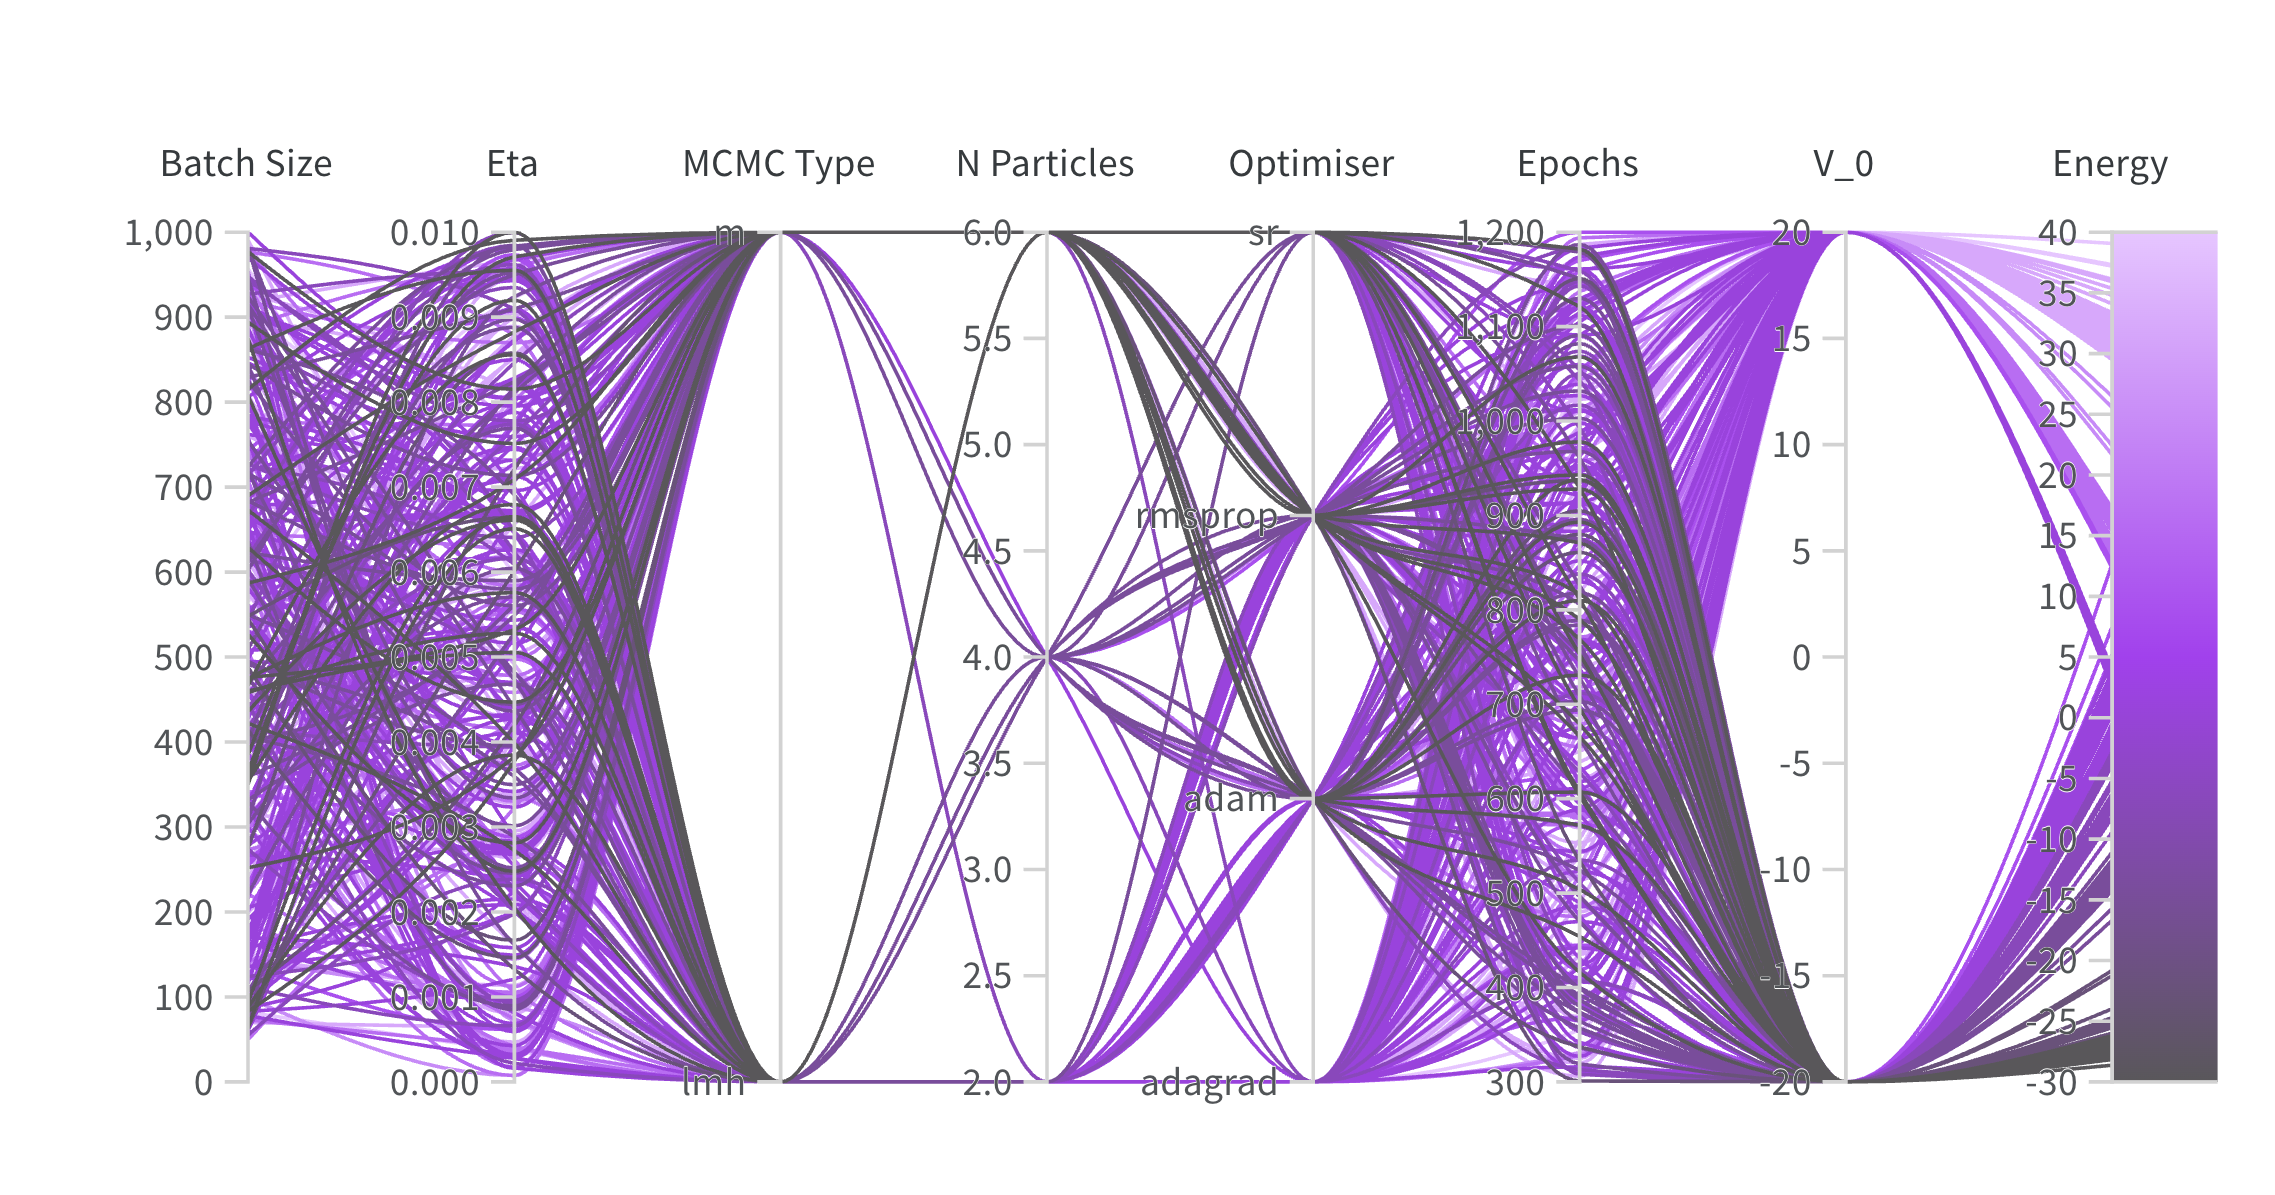
\includegraphics[width=0.8\linewidth]{Chapters/Results/N2/vmc_complete.png}
    \caption{Sweep over 321 hyperparameters for the standard VMC ansatz, from which the results shall be aggregated for the one-dimensional system.}
    \label{fig:rbm_complete_sweep}
\end{figure}

\section{Additional Results 2D Case}\label{apendix:more_results_2d}
\begin{figure}[H]
    \centering
    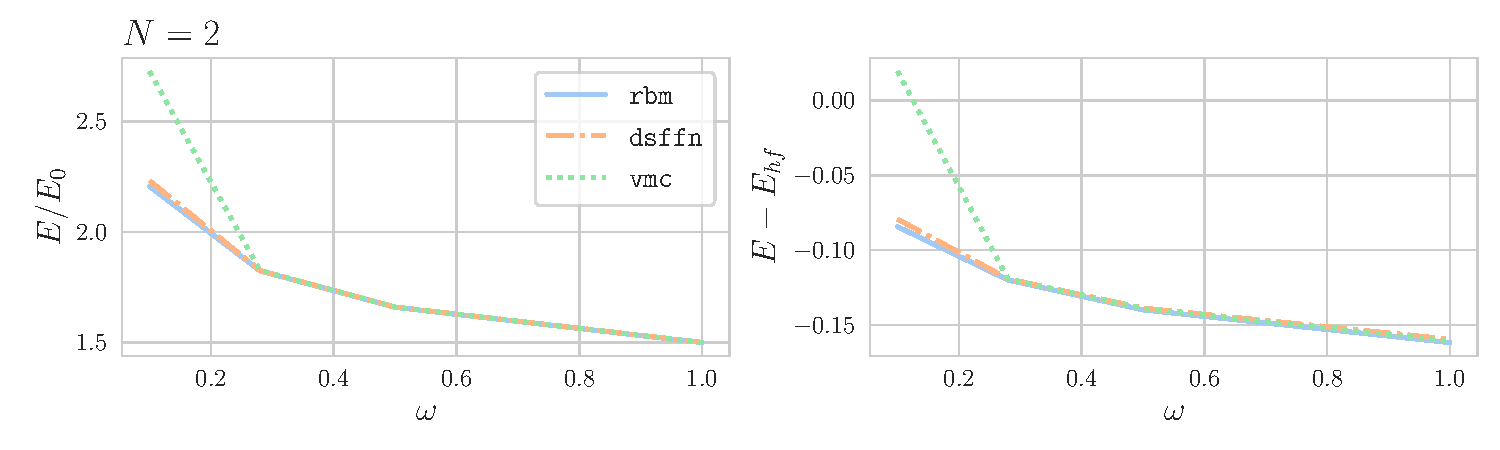
\includegraphics[width=\textwidth]{Chapters/Results/dots/total_energy_vs_omega_n2.pdf}
    \caption{On the left, the energy over non-interactive energy values for two-particle two dimensional quantum dot as a function of frequency of the trap. On the right, the correlation energy with $E_{hf}$ the Hartree-Fock energy.}
\end{figure}


\begin{figure}[H]
    \centering
    \begin{subfigure}[t]{0.32\textwidth}
        \centering
        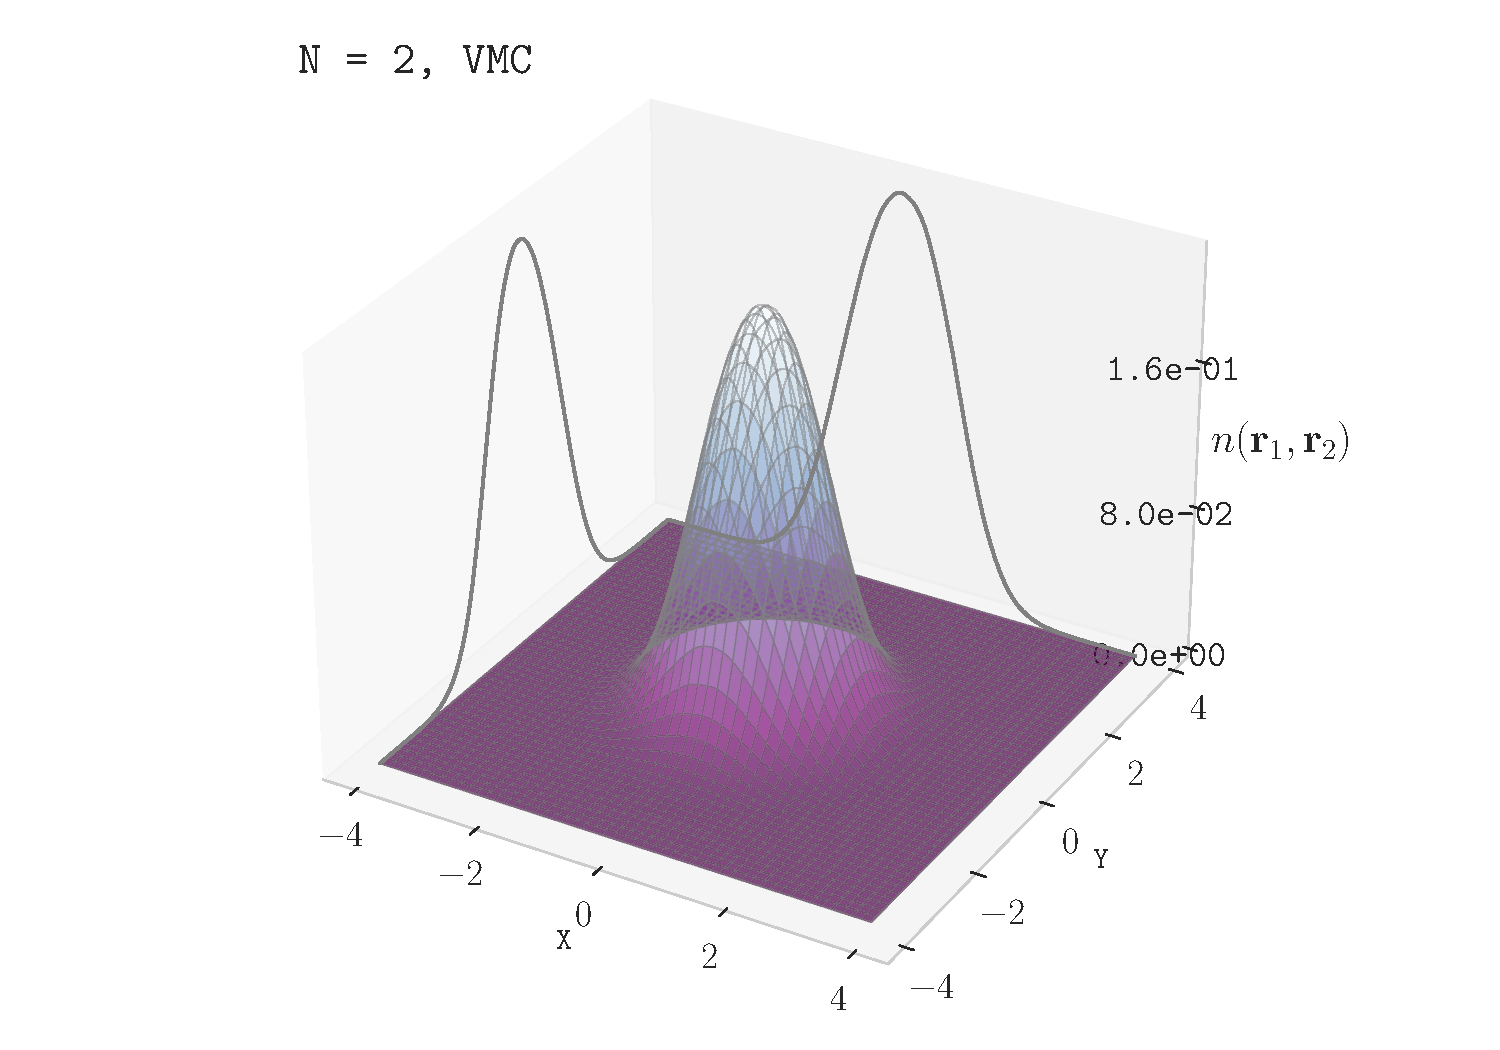
\includegraphics[width=\textwidth]{Chapters/Results/dots/density_profile_3d_N2_nqs_VMC_1.0.pdf}
        \label{fig:sub1}
    \end{subfigure}
    \begin{subfigure}[t]{0.32\textwidth}
        \centering
        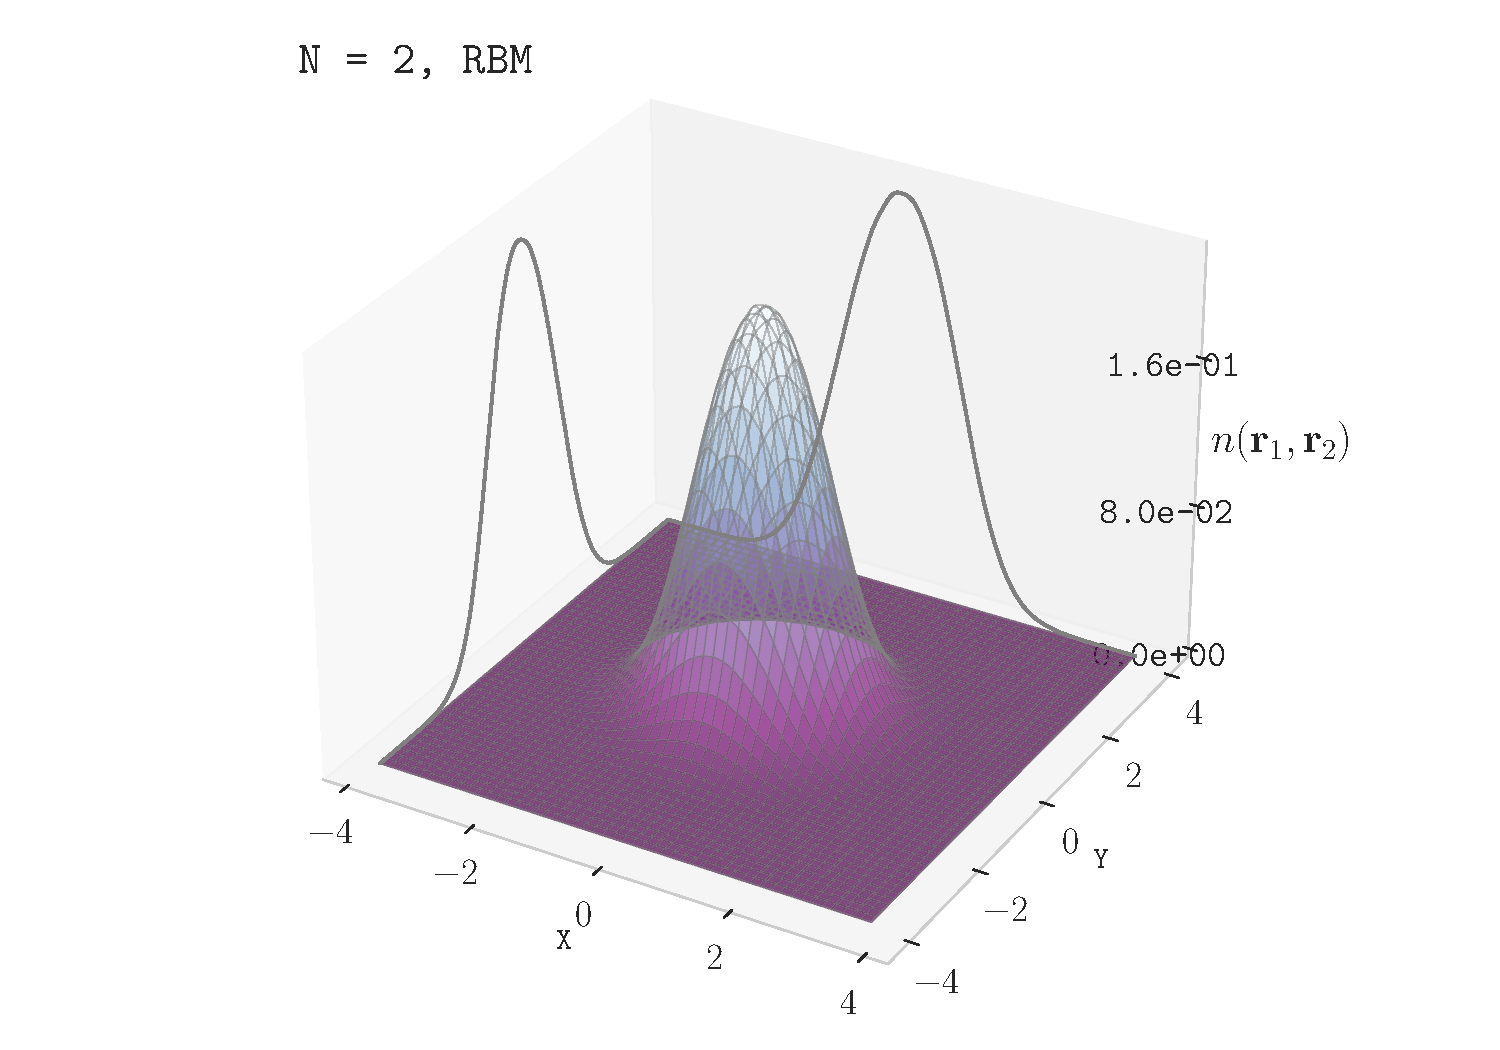
\includegraphics[width=\textwidth]{Chapters/Results/dots/density_profile_3d_N2_nqs_RBM_1.0.pdf}
        \label{fig:sub2}
    \end{subfigure}
    \begin{subfigure}[t]{0.32\textwidth}
        \centering
        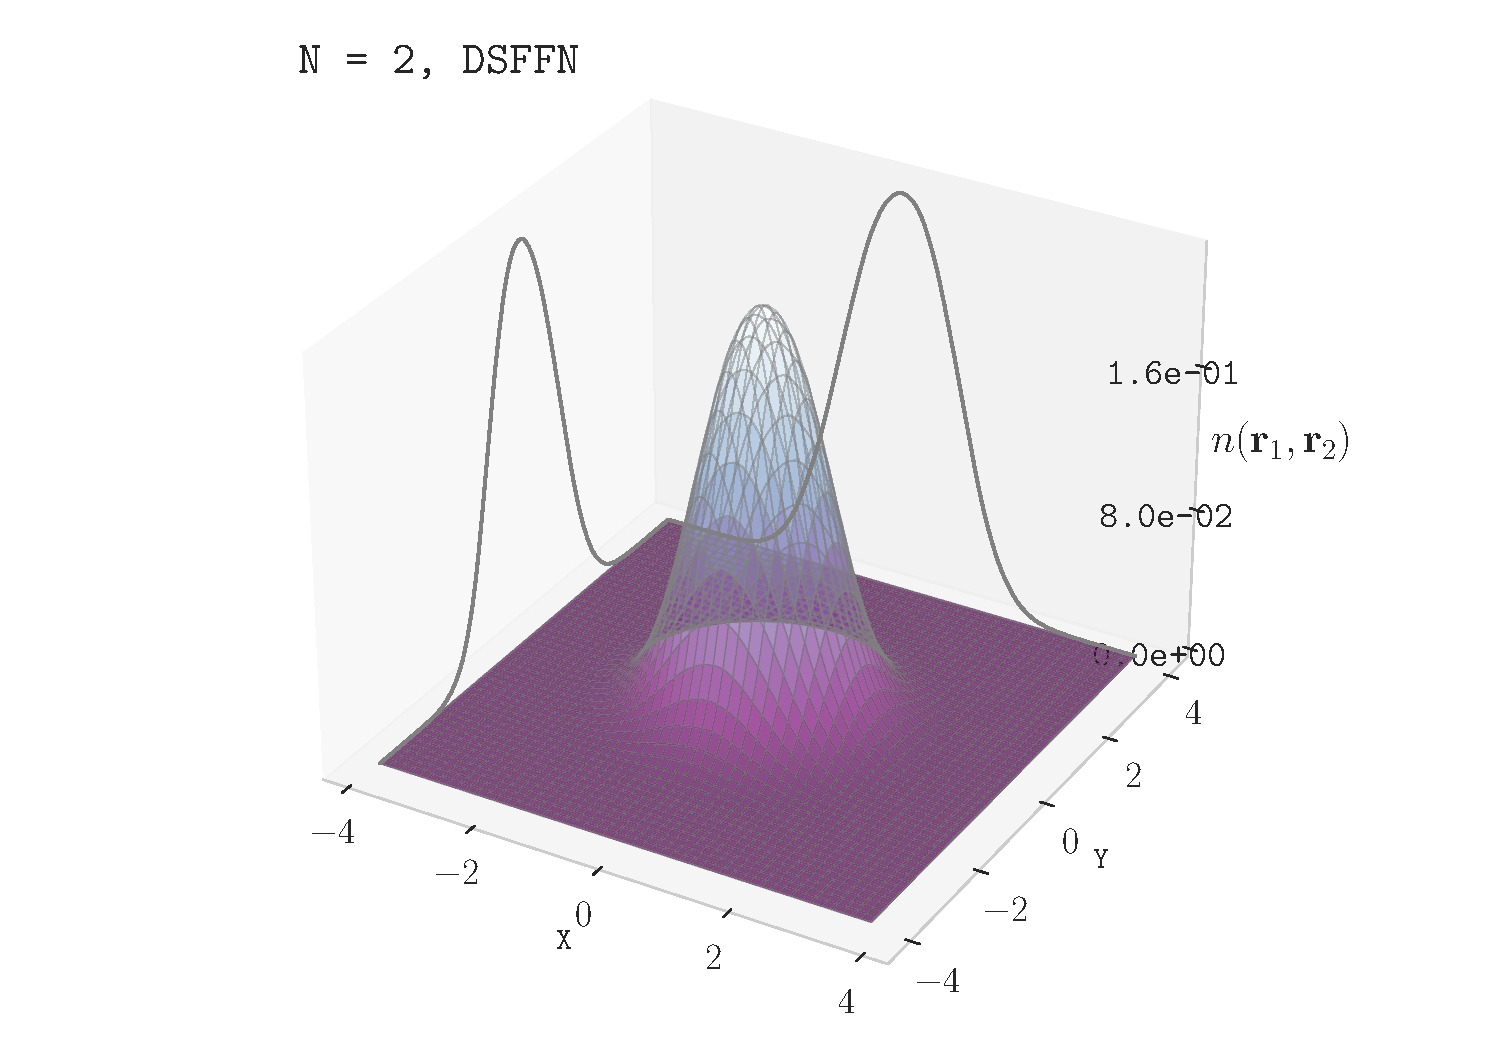
\includegraphics[width=\textwidth]{Chapters/Results/dots/density_profile_3d_N2_nqs_DSFFN_1.0.pdf}
        \label{fig:sub3}
    \end{subfigure}
    \begin{subfigure}[t]{0.32\textwidth}
        \centering
        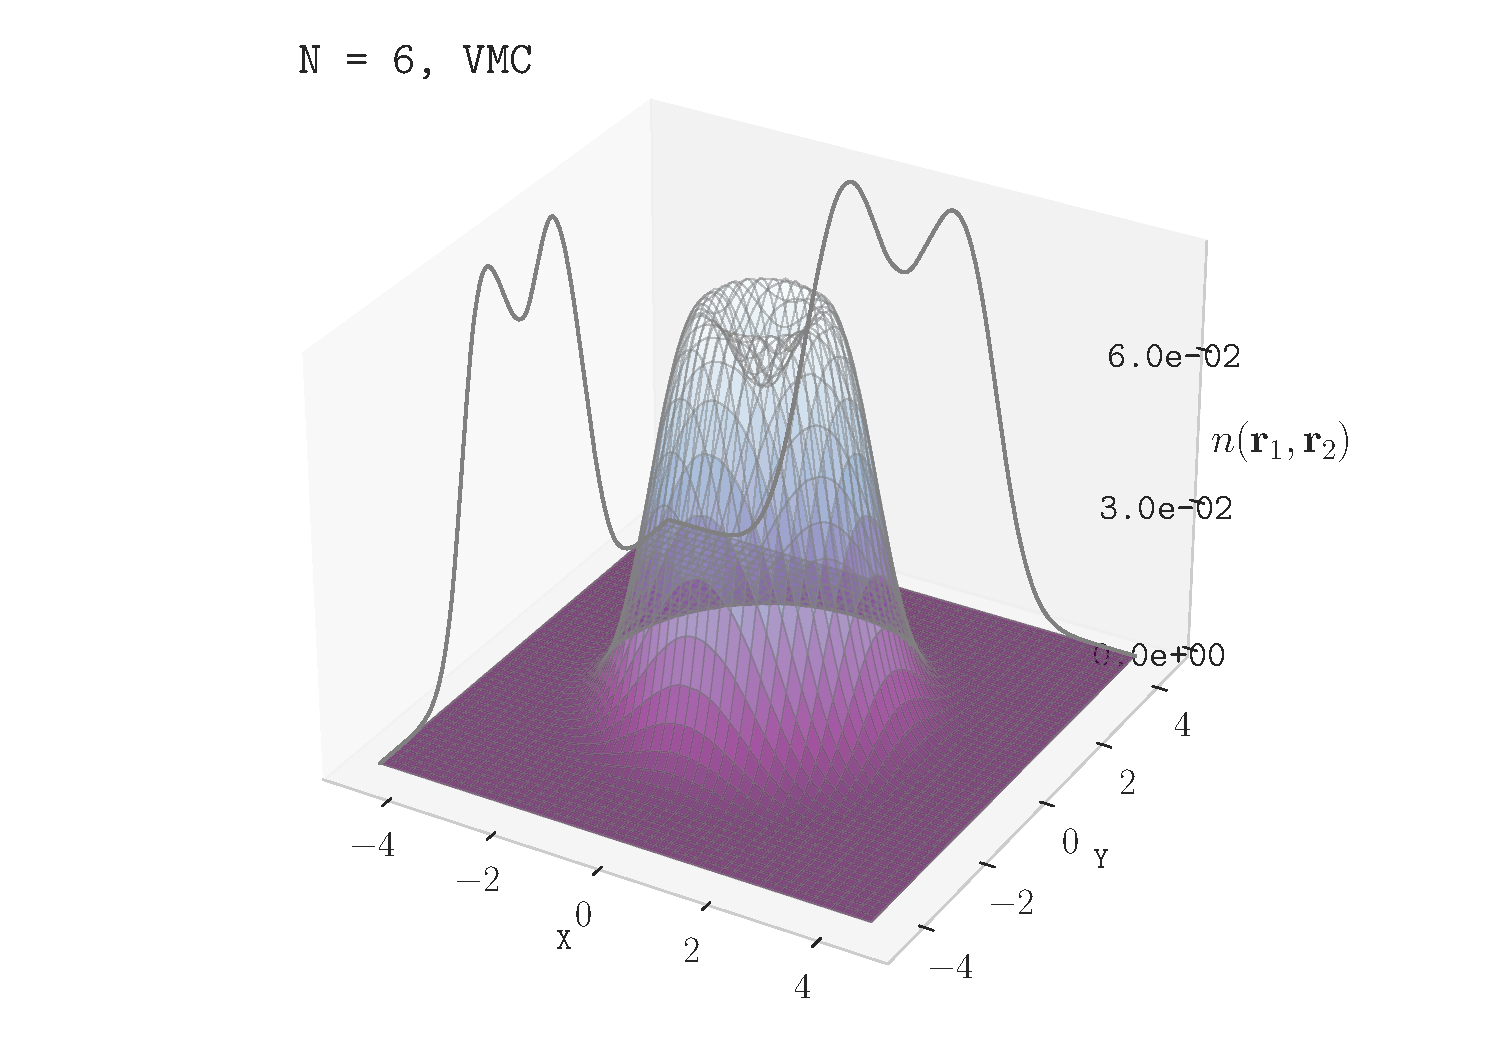
\includegraphics[width=\textwidth]{Chapters/Results/dots/density_profile_3d_N6_nqs_VMC_1.0.pdf}
        \label{fig:sub1}
    \end{subfigure}
    \begin{subfigure}[t]{0.32\textwidth}
        \centering
        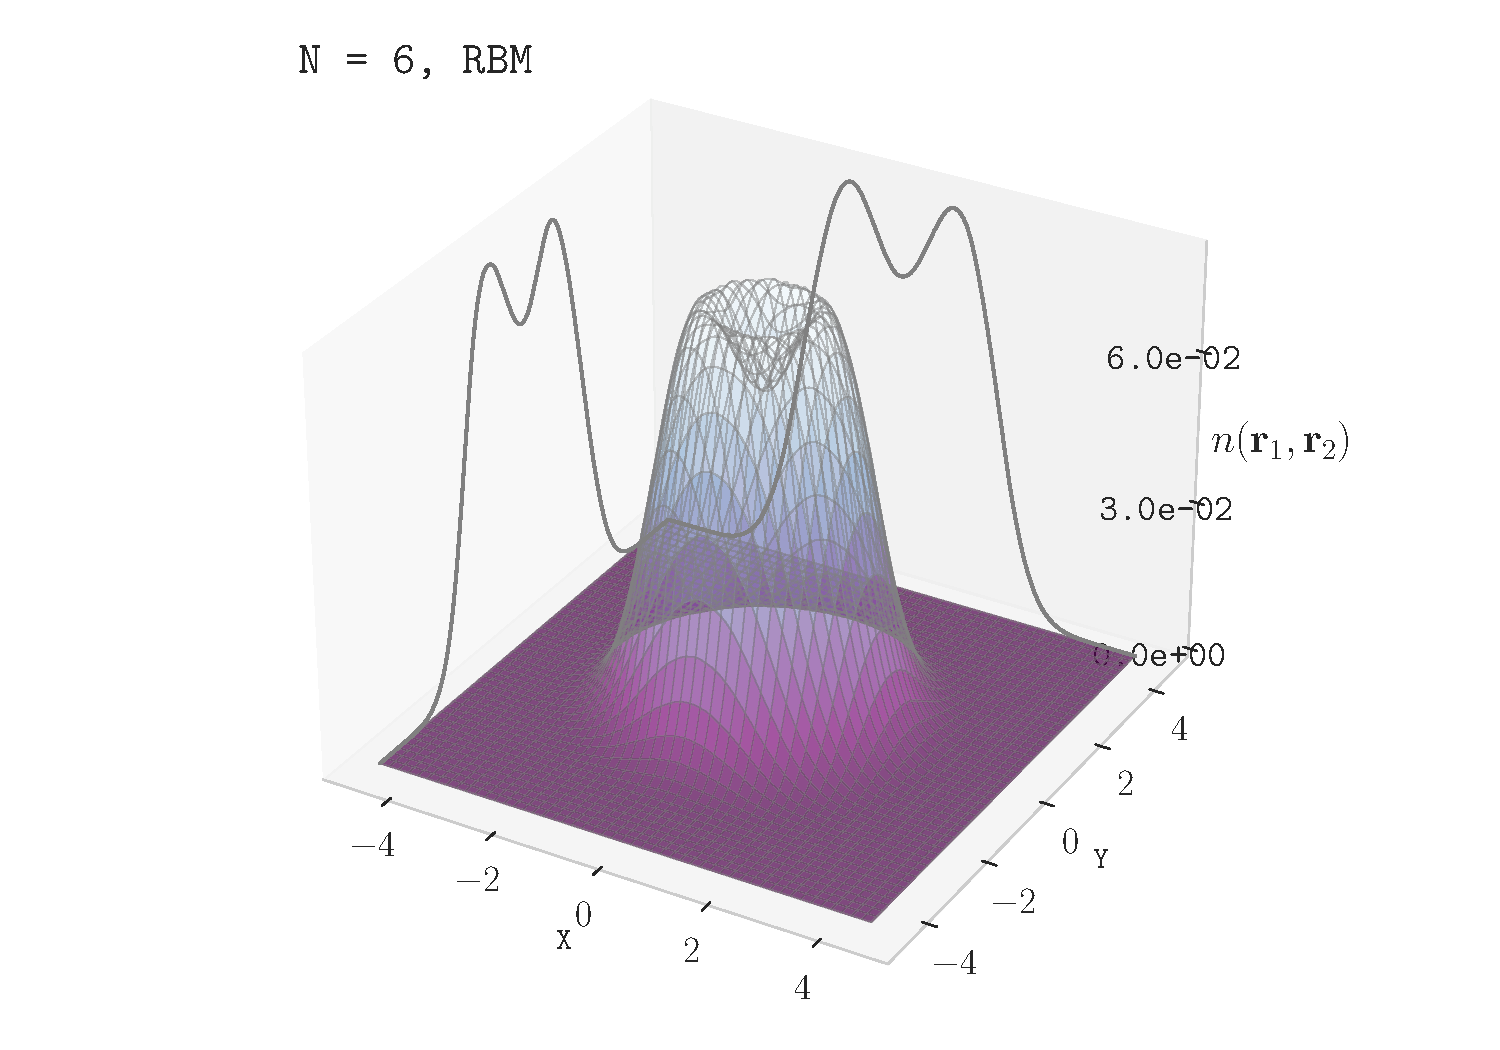
\includegraphics[width=\textwidth]{Chapters/Results/dots/density_profile_3d_N6_nqs_RBM_1.0.pdf}
        \label{fig:sub2}
    \end{subfigure}
    \begin{subfigure}[t]{0.32\textwidth}
        \centering
        \includegraphics[width=\textwidth]{Chapters/Results/dots/density_profile_3d_N6_nqs_dsffn_1.0.pdf}
        \label{fig:sub3}
    \end{subfigure}
    \caption{One-body density for the two and six particle case in a trap frequency of $\omega = 1.0$}
    \label{fig:total}
\end{figure}